\section{Theoretische Grundlage}
\label{sec:Theorie}

Der zweite Hauptsatz der Thermodynamik sagt, dass Wärme von einem wärmeren zu einem kälteren Reservoir fließt. Mithilfe einer Wärmepumpe lässt sich dieser Prozess umkehren. Dazu wird weitere Energie benötigt, zum Beispiel mechanische Arbeit. Ziel des Versuches ist es, eine Aussage über die Qualität der Wärmepumpe zu treffen. Um dies zu realisieren, werden die Güteziffer und der Massendurchsatz untersucht.

\subsection{Güteziffer}
Der erste Hauptsatz der Wärmelehre verlangt, dass die vom Transportmedium an das wärmere Reservoir abgegebene Wärmemenge $Q_\text{1}$ gleich der Summe der aus dem kälteren Reservoir entnommenen Wärmemenge $Q_\text{2}$ und der aufgewendeten Arbeit $A$ ist, also
\begin{equation}
	\label{eqn:Q1}
		Q_\text{1} = Q_\text{2} + A \ .
\end{equation}
Die Güteziffer $\nu$ ist im idealisierten Fall das Verhältnis zwischen der transportierten Wärmemenge $Q_\text{1}$ und der verrichteten mechanischen Arbeit $A$:
\begin{equation}
	\label{eqn:nu}
	\nu_\text{ideal} = \frac{Q_\text{1}}{A} \ .
\end{equation}
Aus dem zweiten Hauptsatz der Thermodynamik lässt sich eine Beziehung zwischen den Wärmemengen $Q_\text{1}$ und $Q_\text{2}$ sowie den Temperaturen $T_\text{1}$ und $T_\text{2}$ der Reservoire herstellen
\begin{equation}
	\label{eqn:reversibel}
	\frac{Q_\text{1}}{T_\text{1}} - \frac{Q_\text{2}}{T_\text{2}} = 0 \ .
\end{equation}
Allerdings ist die Gültigkeit der Formel \ref{eqn:reversibel} an die Forderung, dass die Wärmeübertragung reversibel verläuft, geknüpft. Dies bedeutet, dass der Prozess jederzeit umgekehrt ablaufen kann, wodurch die investierte mechanische Arbeit zurück gewonnen werden kann. Für den realistischen, irreversiblen Fall gilt eine andere Beziehung
\begin{equation}
	\label{eqn:irreversibel}
	\frac{Q_\text{1}}{T_\text{1}} - \frac{Q_\text{2}}{T_\text{2}} > 0 \ .
\end{equation}
Mit den Gleichungen \ref{eqn:Q1} und \ref{eqn:reversibel} folgt nun
\begin{equation}
	Q_\text{1} = A + \frac{T_\text{2}}{T_\text{1}} Q_\text{1}
\end{equation}
und für die Güteziffer einer idealen Wärmepumpe
\begin{equation}
	\nu_\text{ideal} = \frac{Q_\text{1}}{A} = \frac{T_\text{1}}{T_\text{1} - T_\text{2}} \ .
	\label{eqn:nuideal}
\end{equation}
Die Güteziffer für eine reale Wärmepumpe folgt aus \ref{eqn:Q1} und \ref{eqn:irreversibel} zu
\begin{equation}
	\nu_\text{real} < \frac{T_\text{1}}{T_\text{1} - T_\text{2}} \ .
\end{equation}
Die reale Güteziffer wird im folgenden über
\begin{equation}
	\nu_\text{real} = \frac{\Delta Q_\text{1}}{\Delta t N} = (m_\text{1} c_\text{w} + m_\text{k} c_\text{k}) \frac{\Delta T_\text{1}}{\Delta t N}
	\label{eqn:nureal}
\end{equation}
berechnet, wobei $N$ := gemittelte Leistungsaufnahme des Kompressors.

\subsection{Massendurchsatz}
Der Massendurchsatz für die Wärmepumpe berechnet sich nach [1,S.5] über den Differentialquotienten:
\begin{equation}
	\label{eqn:kp1}
	\frac{d Q_\text{2}}{d t} = (m_\text{2} c_\text{w} + m_\text{k} c_\text{k}) \frac{\Delta T_\text{2}}{\Delta t N}
\end{equation}
und
\begin{equation}
	\label{eqn:kp2}
	\frac{d Q_\text{2}}{d t} = L \frac{d m}{d t}
\end{equation}
nach einsetzen von \ref{eqn:kp1} in \ref{eqn:kp2} folgt:
\begin{equation}
	\frac{dm}{dt} = (m_\text{2} c_\text{w} + m_\text{k} c_\text{k}) \frac{\Delta T_\text{2}}{\Delta t L}
	\label{eqn:dm/dt}
\end{equation}
Wobei $L$ := bekannte Verdampfungswärme.

\subsection{Mechanische Kompressorleistung}
Wenn ein Kompressor ein Gasvolumen $V_\text{a}$ auf das Volumen $V_\text{b}$ verringert, leistet dieser die Arbeit $A_\text{m}$
\begin{equation}
	A_\text{m} = - \int_{V_\text{a}}^{V_\text{b}} p \, dV \ .
\end{equation}
Mit der Annahme, dass die Kompression adiabatisch verläuft, gilt die Poissonsche Gleichung:
\begin{equation}
	p_\text{a} V_\text{a}^\kappa = p_\text{b} V_\text{b}^\kappa = p V^\kappa \ .
\end{equation}
Eine adiabatische Zustandsänderung ist ein Prozess, bei dem ein System von einem Zustand in einen anderen übergeht, ohne Wärme mit der Umgebung auszutauschen. \\
Mit der Poissonschen Gleichung und
\begin{align*}
	N_\text{mech} = \frac{dA_\text{m}}{dt} \ ,
\end{align*}
folgt $N_\text{mech}$ zu:
\begin{equation}
	N_\text{mech} = \frac{1}{\kappa - 1} \left(p_\text{b} \sqrt[\kappa]{\frac{p_\text{a}}{p_\text{b}}} - p_\text{a} \right) \frac{1}{\rho} \frac{dm}{dt} \ ,
	\label{eqn:nmech}
\end{equation}
mit der Dichte $\rho$ und dem Druck $p_\text{a}$.

\subsection{Allgemeiner Aufbau einer Wärmepumpe}
Im folgenden wird die prinzipielle Funktionsweise einer Wärmepumpe beschrieben. Diese kann schematisch wie folgt dargestellt werden:
\begin{figure}[H]
	\centering
	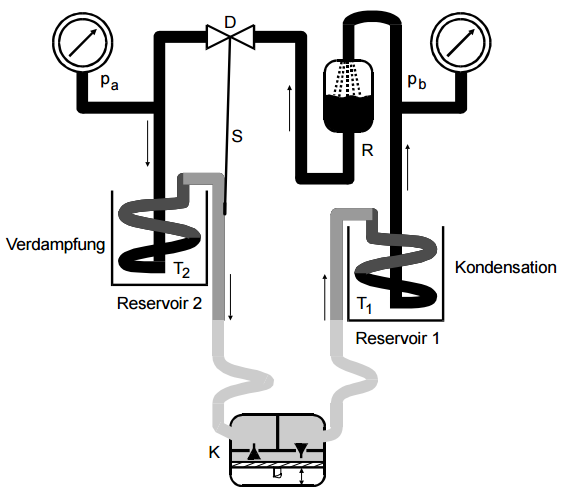
\includegraphics[height=7cm]{Allgemeine_Waermepumpe.png}
	\caption{Allgemeiner Aufbau einer Wärmepumpe [1]}
\end{figure}

Für die Wärmepumpe wird ein reales Gas verwendet, welches Wärme beim Verdampfen aufnimmt und beim Kondensieren wieder abgibt. Die Wärme wird also in Form von Phasenumwandlungsenergie des Gases transportiert. Daraus folgt, dass das verwendete Gas eine hohe Kondensationswärme haben sollte. Der Kompressor $K$ komprimiert das Gas adiabatisch und erzeugt einen Kreislauf des Mediums. Zwischen den Reservoiren ist ein Drosselventil $D$ angebracht, welches das Gas bei einem bestimmten Druck passieren lässt. Dadurch entsteht ein Druckunterschied $p_\text{b} - p_\text{a}$. Das Gas mit dem Druck $p_\text{a}$ und der Temperatur $T_\text{2}$ ist gasförmig, während es auf der anderen Seite bei $p_\text{b}$ mit der Temperatur $T_\text{1}$ flüssig ist. Nachdem das flüssige Medium durch das Druckventil geströmt ist, verdampft dieses im Reservoir 2 und entzieht diesem die Verdampfungswärme $L$ pro Gramm Substanz. Das zweite Reservoir ist damit das kältere und Wärme abgebende Reservoir. In dem Kompressor $K$ wird das Gas komprimiert, wodurch es sich erwärmt. Durch die Erwärmung steigt der Druck $p_\text{a}$ im Reservoir 1, bis sich das Gas verflüssigt, wodurch Wärme an die Umgebung abgegeben wird. \\
Wichtig ist, dass nur Gase in den Kompressor gelangen. Erreicht wird das mit diesen Apparaten:
\begin{itemize}
\item mit dem Reiniger $R$, werden Gasreste und damit Blasen entfernt
\item mit der Steuervorrichtung $S$, die das Drosselventil $D$ reguliert
\end{itemize}

\newpage
\subsection{Fehlerrechnung}
Sämtliche Fehlerrechnungen werden mit Hilfe von Python 3.4.3 durchgeführt.
\subsubsection{Mittelwert}
Der Mittelwert einer Messreihe $x_\text{1}, ... ,x_\text{n}$ lässt sich durch die Formel
\begin{equation}
	\overline{x} = \frac{1}{N} \sum_{\text{k}=1}^\text{N} x_\text{k}
	\label{eqn:ave}
\end{equation}
berechnen. Die Standardabweichung des Mittelwertes beträgt
\begin{equation}
	\Delta \overline{x} = \sqrt{ \frac{1}{N(N-1)} \sum_{\text{k}=1}^\text{N} (x_\text{k} - \overline{x})^2}
	\label{eqn:var}
\end{equation}

\subsubsection{Gauß'sche Fehlerfortpflanzung}
Wenn $x_\text{1}, ..., x_\text{n}$ fehlerbehaftete Messgrößen im weiteren Verlauf benutzt werden, wird der neue Fehler $\Delta f$ mit Hilfe der Gaußschen Fehlerfortpflanzung angegeben.
\begin{equation}
	\Delta f = \sqrt{\sum_{\text{k}=1}^\text{N} \left( \frac{ \partial f}{\partial x_\text{k}} \right) ^2 \cdot (\Delta x_\text{k})^2}
\end{equation}

\subsubsection{Lineare Regression}
Die Steigung und y-Achsenabschnitt einer Ausgleichsgeraden werden gegebenfalls mittels Linearen Regression berechnet.
\begin{equation}
	y = m \cdot x + b
\end{equation}
\begin{equation}
	m = \frac{ \overline{xy} - \overline{x} \overline{y} } {\overline{x^2} - \overline{x}^2}
\end{equation}
\begin{equation}
	b = \frac{ \overline{x^2}\overline{y} - \overline{x} \, \overline{xy}} { \overline{x^2} - \overline{x}^2}
\end{equation}
\newpage
